%%% GuardLLM threat model: trust boundaries and the session-risk loop
%%%
%%% Purpose: show what crosses each boundary and what does not.
%%%   - Party crossings (1) ingress, (2) model, (4) egress are arrows between regions.
%%%   - Internal gates (3) authorization/integrity never move data across a boundary.
%%%   - Retained session state sits in the centre with four edges: two writes,
%%%     two reads. Those four edges are the loop.
%%%
%%% Compile: pdflatex threat_model.tex
%%% SVG:     dvisvgm --pdf --no-fonts --output=threat_model.svg threat_model.pdf
%%%
%%% Palette matches local/guardllm-diagram.tex so the docs figure and the paper
%%% figure read as one system.

\documentclass[border=12pt]{standalone}
\usepackage{tikz}
\usetikzlibrary{arrows.meta, positioning, calc, fit, backgrounds}

% Fill the page instead of leaving it transparent. Without this the PDF and the
% SVG carry no background at all, which reads correctly on a white page and is
% largely illegible on GitHub in dark mode: the figure's own text is near-black
% and the window behind it is too. The diagram is designed on white, so it says
% white rather than inheriting whatever sits behind it.
%
% NOT the standalone `bgcolor` option, which that class does not define: it is
% accepted silently and dropped with an "Unused global option" warning, so the
% rebuild looks like it worked and the background is still transparent.
\pagecolor{white}
\usepackage[T1]{fontenc}
\usepackage{lmodern}

\definecolor{clTrusted}{HTML}{2E7D32}
\definecolor{clUntrusted}{HTML}{C62828}
\definecolor{clMeta}{HTML}{1565C0}
\definecolor{clOrange}{HTML}{E65100}
\definecolor{clGray}{HTML}{37474F}
\definecolor{clLightGray}{HTML}{546E7A}
\definecolor{clLLMfill}{HTML}{C5CAE9}
\definecolor{clLLMborder}{HTML}{283593}
\definecolor{clStateFill}{HTML}{E3F2FD}
\definecolor{clZoneApp}{HTML}{F5F7F8}
\definecolor{clZoneLLM}{HTML}{E8EAF6}

\begin{document}
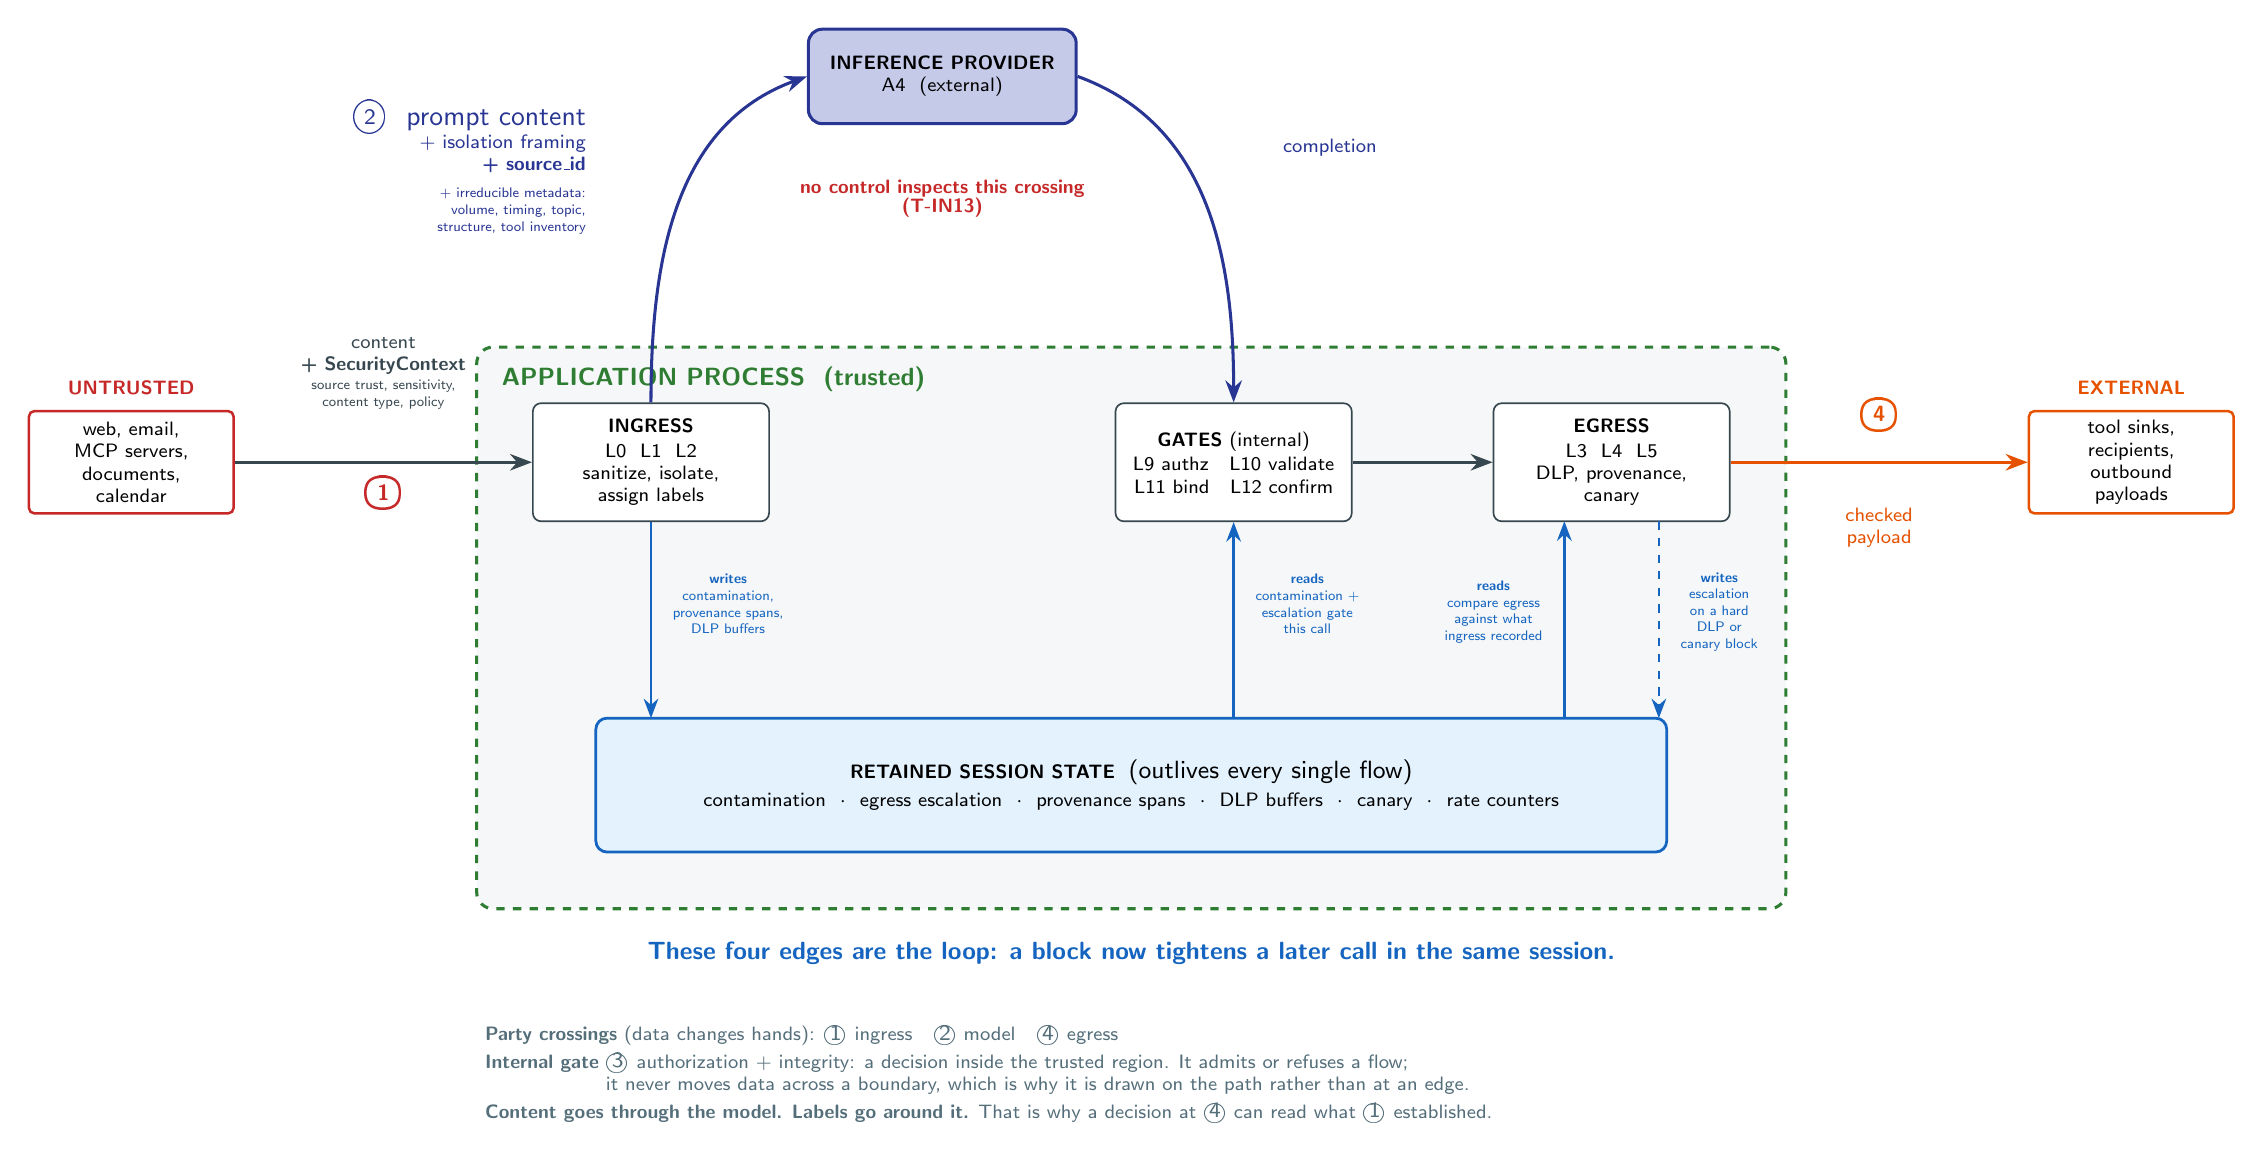
\begin{tikzpicture}[
    >=Stealth,
    font=\sffamily\small,
    ctrl/.style={draw=clGray, fill=white, rounded corners=3pt,
      minimum width=3.0cm, minimum height=1.5cm, align=center,
      font=\sffamily\scriptsize, line width=0.6pt},
    ext/.style={draw, rounded corners=2pt, fill=white,
      minimum width=2.6cm, minimum height=1.3cm, align=center,
      font=\sffamily\scriptsize, line width=0.9pt},
    flow/.style={->, clGray, line width=1.1pt},
    lbl/.style={font=\sffamily\scriptsize, align=center, clGray},
    xing/.style={font=\sffamily\scriptsize\bfseries, align=center},
    meta/.style={->, clMeta, line width=0.9pt},
    metalbl/.style={font=\sffamily\tiny, align=center, clMeta},
    every path/.style={line width=0.6pt},
  ]

  % ==========================================================
  % Internal nodes (placed first so the app zone can fit them)
  % ==========================================================
  \node[ctrl] (ingress) at (3.0, 6.4)
    {\textbf{INGRESS}\\[1pt] L0 \ L1 \ L2\\ sanitize, isolate,\\ assign labels};

  \node[ctrl] (gates) at (10.4, 6.4)
    {\textbf{GATES} \scriptsize(internal)\\[1pt] L9 authz \ \ L10 validate\\ L11 bind \ \ L12 confirm};

  \node[ctrl] (egress) at (15.2, 6.4)
    {\textbf{EGRESS}\\[1pt] L3 \ L4 \ L5\\ DLP, provenance,\\ canary};

  \node[draw=clMeta, fill=clStateFill, rounded corners=4pt, line width=1.0pt,
        minimum width=13.6cm, minimum height=1.7cm, align=center,
        font=\sffamily\scriptsize] (state) at (9.1, 2.3)
    {\textbf{RETAINED SESSION STATE} \ \small(outlives every single flow)\\[2pt]
     contamination \ $\cdot$ \ egress escalation \ $\cdot$ \ provenance spans
     \ $\cdot$ \ DLP buffers \ $\cdot$ \ canary \ $\cdot$ \ rate counters};

  % ==========================================================
  % Application process boundary
  % ==========================================================
  \begin{scope}[on background layer]
    \node[draw=clTrusted, dashed, line width=1.1pt, rounded corners=6pt,
          fill=clZoneApp, inner sep=20pt,
          fit=(ingress)(gates)(egress)(state)] (app) {};
  \end{scope}
  \node[font=\sffamily\small\bfseries, clTrusted, anchor=north west]
    at ([xshift=6pt, yshift=-4pt]app.north west) {APPLICATION PROCESS \ (trusted)};

  % ==========================================================
  % External parties
  % ==========================================================
  \node[ext, draw=clUntrusted] (src) at (-3.6, 6.4)
    {web, email,\\ MCP servers,\\ documents,\\ calendar};
  \node[font=\sffamily\scriptsize\bfseries, clUntrusted, above=2pt of src]
    {UNTRUSTED};

  \node[draw=clLLMborder, fill=clLLMfill, rounded corners=5pt, line width=1.1pt,
        minimum width=3.4cm, minimum height=1.2cm, align=center,
        font=\sffamily\scriptsize] (llm) at (6.7, 11.3)
    {\textbf{INFERENCE PROVIDER}\\ A4 \ (external)};

  \node[ext, draw=clOrange] (sink) at (21.8, 6.4)
    {tool sinks,\\ recipients,\\ outbound\\ payloads};
  \node[font=\sffamily\scriptsize\bfseries, clOrange, above=2pt of sink]
    {EXTERNAL};

  % ==========================================================
  % (1) INGRESS crossing
  % ==========================================================
  \draw[flow] (src.east) -- (ingress.west);
  \node[xing, clUntrusted] at ($(src.east)!0.5!(ingress.west)+(0,-0.45)$)
    {\large\textcircled{\footnotesize 1}};
  \node[lbl, anchor=south] at ($(src.east)!0.5!(ingress.west)+(0,0.55)$)
    {content \\ \textbf{+ SecurityContext}\\[-1pt]
     \tiny source trust, sensitivity,\\[-2pt] \tiny content type, policy};

  % ==========================================================
  % (2) MODEL crossing -- the uninspected one
  % ==========================================================
  \draw[flow, clLLMborder] (ingress.north) to[out=90, in=200] (llm.west);
  \draw[flow, clLLMborder] (llm.east) to[out=340, in=90] (gates.north);

  \node[lbl, clLLMborder, align=right, anchor=north east] at (2.3, 11.0)
    {\large\textcircled{\footnotesize 2}\normalsize\ \ prompt content\\ + isolation framing\\
     \textbf{+ source\_id}\\[2pt]
     \tiny + irreducible metadata:\\[-2pt] \tiny volume, timing, topic,\\[-2pt]
     \tiny structure, tool inventory};
  \node[lbl, clLLMborder, anchor=west] at (10.9, 10.4) {completion};

  \node[font=\sffamily\scriptsize\bfseries, clUntrusted, align=center]
    at (6.7, 9.75)
    {no control inspects this crossing\\[-1pt] \scriptsize (T-IN13)};

  % ==========================================================
  % (4) EGRESS crossing
  % ==========================================================
  \draw[flow] (gates.east) -- (egress.west);
  \draw[flow, clOrange] (egress.east) -- (sink.west);
  \node[xing, clOrange] at ($(egress.east)!0.5!(sink.west)+(0,0.55)$)
    {\large\textcircled{\footnotesize 4}};
  \node[lbl, clOrange, anchor=north] at ($(egress.east)!0.5!(sink.west)+(0,-0.45)$)
    {checked\\ payload};

  % ==========================================================
  % The loop: four edges on the session state
  % ==========================================================
  % write 1: ingress labels the session
  \draw[meta] (ingress.south) -- (3.0, 3.15);
  \node[metalbl, anchor=west] at (3.15, 4.6)
    {\textbf{writes}\\ contamination,\\ provenance spans,\\ DLP buffers};

  % read 1: egress checks consult retained labels
  \draw[meta] (14.6, 3.15) -- (14.6, 5.65);
  \node[metalbl, anchor=east] at (14.45, 4.5)
    {\textbf{reads}\\ compare egress\\ against what\\ ingress recorded};

  % write 2: the backward edge -- an egress block escalates the session
  \draw[meta, dashed] (15.8, 5.65) -- (15.8, 3.15);
  \node[metalbl, anchor=west] at (15.95, 4.5)
    {\textbf{writes}\\ escalation\\ on a hard\\ DLP or\\ canary block};

  % read 2: gates tighten for a LATER call
  \draw[meta] (10.4, 3.15) -- (gates.south);
  \node[metalbl, anchor=west] at (10.55, 4.6)
    {\textbf{reads}\\ contamination +\\ escalation gate\\ this call};

  \node[font=\sffamily\small\bfseries, clMeta, align=center, anchor=north]
    at ([yshift=-8pt]app.south)
    {These four edges are the loop: a block now tightens a \emph{later} call in the same session.};

  % ==========================================================
  % Legend: crossings vs gates
  % ==========================================================
  \node[align=left, font=\sffamily\scriptsize, clLightGray, anchor=north west]
    at ([yshift=-38pt]app.south west)
    {\textbf{Party crossings} (data changes hands):
       \textcircled{\footnotesize 1} ingress \ \
       \textcircled{\footnotesize 2} model \ \
       \textcircled{\footnotesize 4} egress\\[2pt]
     \textbf{Internal gate} \textcircled{\footnotesize 3} authorization + integrity:
       a decision inside the trusted region. It admits or refuses a flow;\\
       \phantom{\textbf{Internal gate} }it never moves data across a boundary,
       which is why it is drawn on the path rather than at an edge.\\[2pt]
     \textbf{Content goes through the model. Labels go around it.}
       That is why a decision at \textcircled{\footnotesize 4} can read what
       \textcircled{\footnotesize 1} established.};

\end{tikzpicture}
\end{document}
